\documentclass[11pt]{article}
\usepackage{tikz}

\usetikzlibrary{arrows}

\begin{document}

\section*{FSM for server}
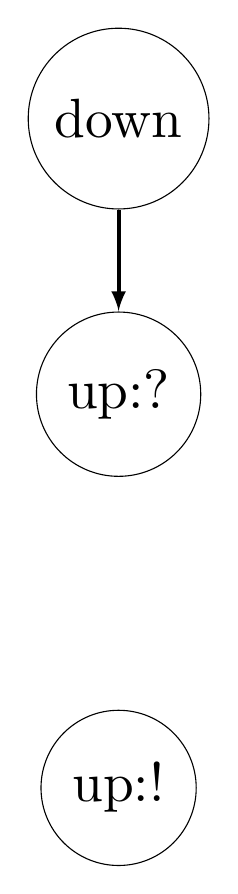
\begin{tikzpicture}
\node[draw, circle, scale=2] at (0,8.5) (down) {down};
\node[draw, circle, scale=2] at (0,5) (upUk) {up:?};
\node[draw, circle, scale=2] at (0,0) (upK) {up:!};

\draw[arrows={-latex}, line width=.5mm, scale=2] (down) to (upUk);
\end{tikzpicture}

\pagebreak

\section*{FSM for receiver}
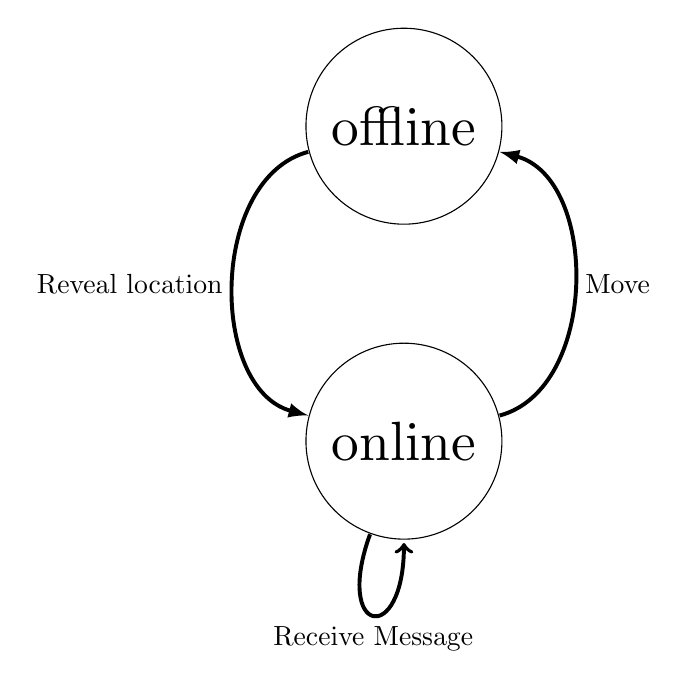
\begin{tikzpicture}
\node[draw, circle, scale=2] at (0,4) (off) {offline};
\node[draw, circle, scale=2] at (0,0) (on) {online};
\draw[arrows={-latex}, line width=.5mm, scale=2] (off) to [out=195, in=165]
  node[left] {Reveal location} (on);
%self edge
\path[arrows={-latex}, out=250, in=270, distance=30mm, line width=.5mm]
  (on) edge[loop] node[below] {Receive Message} (on);
\draw[arrows={-latex}, line width=.5mm, scale=2] (on) to [out=15, in=-15]
  node[right] {Move} (off);
\end{tikzpicture}

\subsection*{Reveal location}
Receiver makes an initial connection to Server, bootstraping the message
channel.
\subsection*{Receive Message}
Server sends a message to Receiver via the message channel and authenticates
it.
\subsection*{Move}
The Receiver moves, connecting to a different network or otherwise not
listening on the message channel.


\end{document}
